\section{Experimental Results}\label{sec:exp}
\subsection{Experimental Setup}\label{sec:exp_setup8}
In order to test and benchmark the code we stored each major benchmark revision in a separate folder. Then we run a script that compiled the code and benchmarked it against $5$ different image sizes (figure \ref{tab:images}). The image sizes were chosen in such a way that they represent real world applications used in an image processing or video processing software. The images \texttt{bhudda\_200.png} and \texttt{bhudda\_300.png} have been chosen since both fit into the L3 cache. 
\begin{figure}
\centering
{\small
\begin{tabular}{rll}
\textbf{Image} & \textbf{Size}\\
\texttt{bhudda\_200.png} & $0.02$ & Megapixel\\
\texttt{bhudda\_320.png} & $0.07$ & Megapixel\\
\texttt{bhudda\_640.png} & $0.26$ & Megapixel\\
\texttt{bhudda\_720p.png} & $0.92$ & Megapixel\\
\texttt{bhudda\_1080p.png} & $2.07$ & Megapixel\\
\end{tabular}
}
\caption{Images used for benchmarking}
\label{tab:images}
\end{figure}

\subsubsection{Platform}
Benchmarking was done on Ubuntu Linux 12.10 running on a Intel Core i7-3610QM "Ivy Bridge" CPU. In order to generate reproducible results the CPU frequency was fixed to $2.3$ GHz with Turbo Boost disabled.
\subsubsection{Tools and counters used}
The code was both compiled and executed on GCC 4.6.4 and ICC 13.1.2.183 64bit. We found that the compiler flags \lstinline{-O3 -march=corei7} produced optimal results in our case. In the results shown we only show results obtained with GCC since the ICC results show the same performance measurements. We noticed that code generated with the compiler flags \lstinline{-O3 -march=corei7-avx} was slower. Since the compiler used the \lstinline{vaddps} instruction with 3 input values. Whereas the \lstinline{-O3 -march=corei7} only add the \lstinline{addps} instruction which uses 2 input values and thus reduces the code size and helps with branch miss predictions since there's less code to load. 

To measure the performance we used a custom timing framework using RTDSC counters. For additional checks we used Intel VTune 2013\footnote{\url{http://software.intel.com/en-us/intel-vtune-amplifier-xe}}. In order to generate the roofline plots (figure \ref{roofline}) we used the perfplot tool\footnote{\url{https://github.com/GeorgOfenbeck/perfplot}} provided by Georg Ofenbeck. To measure the memory bandwith of the reference computer we used Bandwith\footnote{\url{http://zsmith.co/bandwidth.html}}.
\subsection{Results}
We were able to achieve a speedup of $1.98$ for the cache based image \texttt{bhudda\_320.png} with a performance of $0.38$ flops/cycle and a speedup $2.24$ for our HD style image \newline\texttt{bhudda\_1080p.png} with a total performance of $0.32$ flops/cycle (figure \ref{performance}). In our roofline plot \cite{Williams:2009:RIV:1498765.1498785} (figure \ref{roofline}) we observe that we read/write bound for our \texttt{bhudda\_1080p.png} image denoted as \textbf{1080} in the plot. As soon as we decrease the image size (\textbf{720} denotes the image \texttt{bhudda\_720p.png}, \textbf{640} denotes the image \texttt{bhudda\_640.png}, \textbf{320} denotes the image \texttt{bhudda\_320.png}, \textbf{200} denotes the image \texttt{bhudda\_200.png}) we observe that the operational intensity changes but not the performance of the code (figure \ref{roofline}). Hence there must be another limiting factor. 

\setlength\fboxsep{0pt}
\setlength\fboxrule{0.5pt}
 
\begin{figure}\vspace{-10mm}
  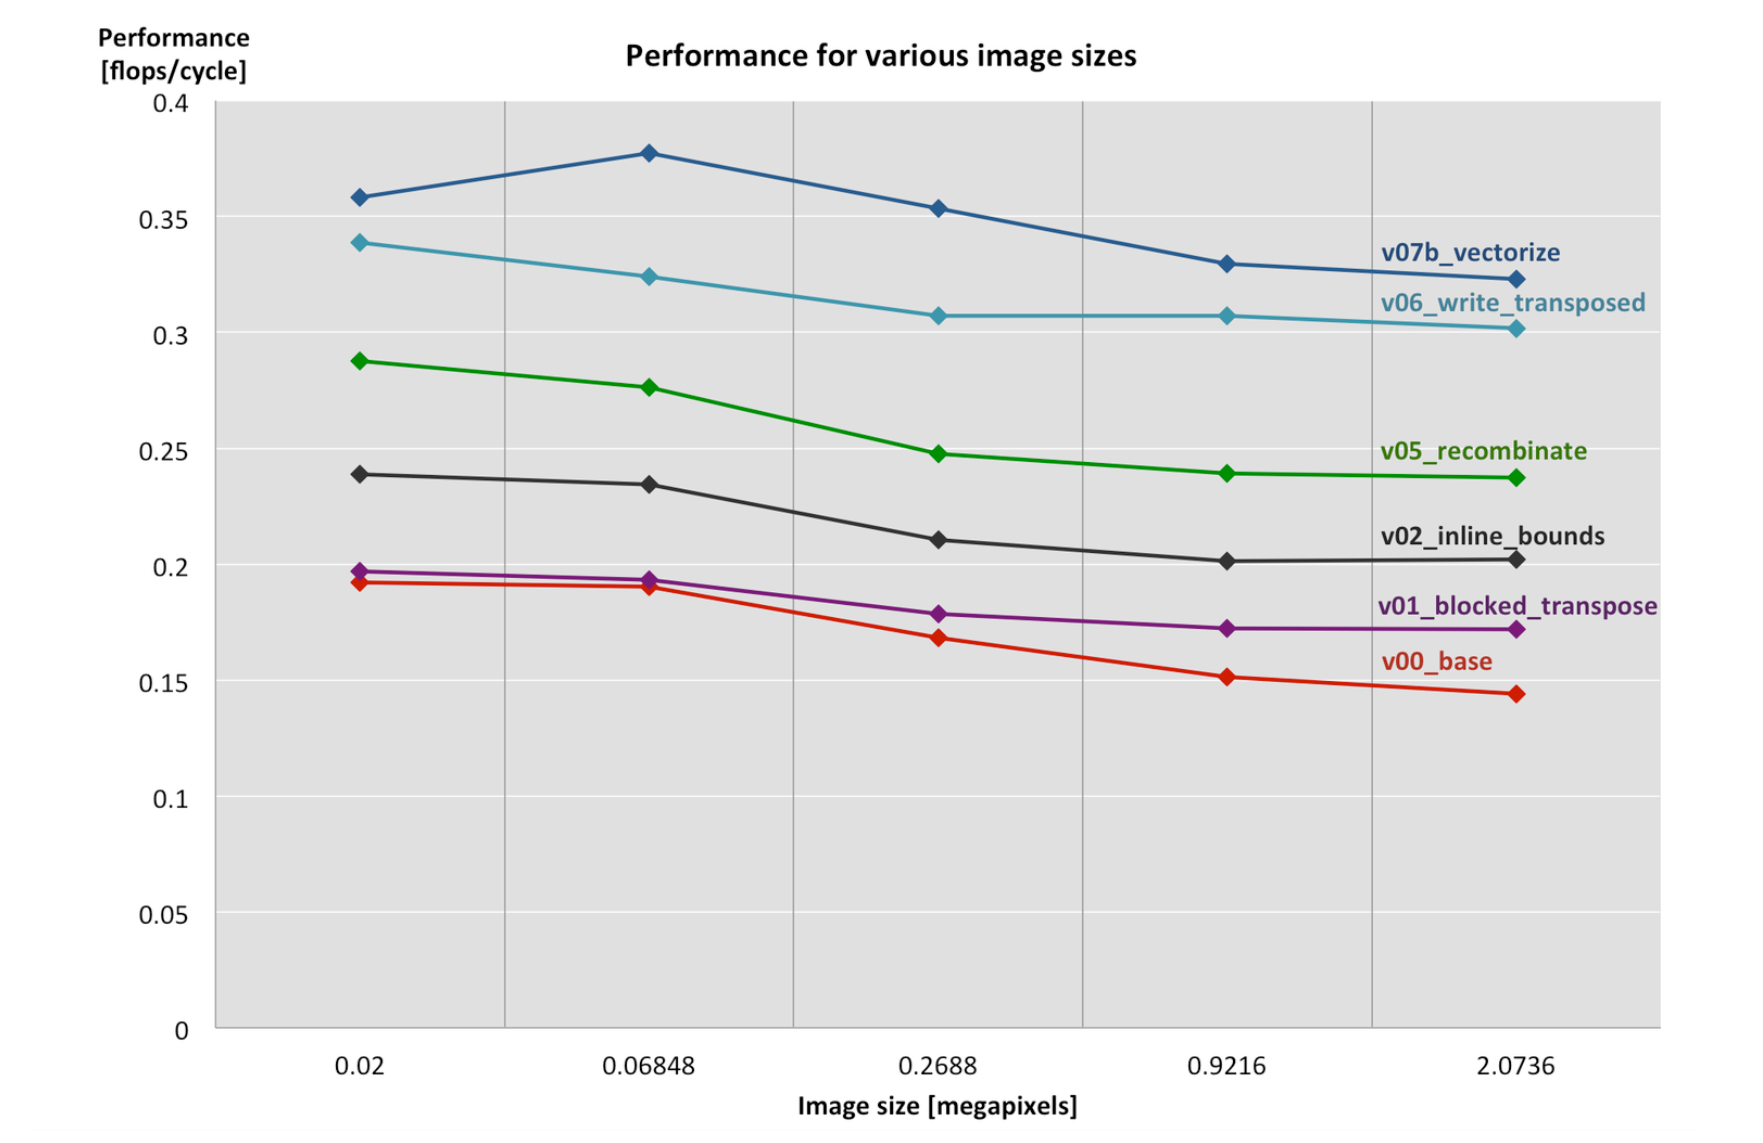
\includegraphics[trim=10mm 0mm 10mm 0mm, clip, width=0.49\textwidth]{figures/performance}
  \caption{Performance plot comparing our different optimisation levels. Compiler: GCC 4.6.4, flags: \lstinline{-O3 -march=corei7}.\label{performance}}
\end{figure}
 
\begin{figure}\vspace{-6mm}\hspace{-5mm}
%  \includegraphics[trim=10mm 0mm 10mm 0mm, clip, width=0.49\textwidth]{figures/roofline}
  \includegraphics[width=0.55\textwidth]{figures/roofline}
  \caption{Roofline plot showing the performance of our vectorised code. .\label{roofline}}
\end{figure}

\comment{ Compiler: GCC 4.6.4, flags: \lstinline{-O3 -march=corei7} }


\comment{
Here you evaluate your work using experiments. You start again with a
very short summary of the section. The typical structure follows.

\mypar{Experimental setup} Specify the platform (processor, frequency, cache sizes)
as well as the compiler, version, and flags used. I strongly recommend that you play with optimisation flags and consider also icc for additional potential speedup.

Then explain what input you used and what range of sizes. The idea is to give enough information so the experiments are reproducible by somebody else on his or her code.

\mypar{Results}
Next divide the experiments into classes, one paragraph for each. In the simplest case you have one plot that has the size on the x-axis and the performance on the y-axis. The plot will contain several lines, one for each relevant code version. Discuss the plot and extract the overall performance gain from baseline to best code. Also state the percentage of peak performance for the best code. Note that the peak may change depending on the situation. For example, if you only do additions it would be 12 Gflop/s
on one core with 3 Ghz and SSE and single precision floating point.

Do not put two performance lines into the same plot if the operations count changed significantly (that's apples and oranges). In that case first perform the optimisations that reduce op count and report the runtime gain in a plot. Then continue to optimise the best version and show performance plots.

{\bf You should}
\begin{itemize}
\item Follow the guide to benchmarking presented in class, in particular
\item very readable, attractive plots (do 1 column, not 2 column plots
for this class), proper readable font size. An example is below (of course you can have a different style),
\item every plot answers a question, which you pose and extract the
answer from the plot in its discussion
\end{itemize}
Every plot should be discussed (what does it show, which statements do
you extract).
}